\documentclass{beamer}
\newif\ifplacelogo
\placelogotrue
\mode<presentation>{\usetheme{Boadilla2}}

\usepackage{geometry}
\usepackage{color}
\usepackage{graphicx}

\usepackage[T1]{fontenc}
\usepackage{fontspec}
\setmainfont{CenturyGothic}
\setsansfont{CenturyGothic}

\AtBeginSection[]{\frame{\tableofcontents[currentsection]}}

\definecolor{myturquoise}{RGB}{0,176,176}
\definecolor{mylightturquoise}{RGB}{54,216,216}


\begin{document}


\setlength{\unitlength}{1mm}
\title{DS Visualisation and Analysis}
\author[Abbey Waldron]{Abbey Waldron}
\date[October 30th, 2015]{}




\setbeamertemplate{navigation symbols}{}

{
\placelogofalse
\begin{frame}
  \titlepage
\end{frame}
}


\begin{frame}{Today}

\begin{itemize}
\item Project hand in start
\item Exam preparation
\item Project presentations start
\end{itemize}

\end{frame}



\begin{frame}{Final Projects}

Please hand it in now - the sooner you hand it in the sooner you can leave.

\vspace{5mm}

Final deadline for hand in is 11:20 am today.

\vspace{5mm}

Do not leave before you have given your presentation to me!

\end{frame}


\begin{frame}{Exam}

\end{frame}


\begin{frame}{Types of Questions}

\begin{itemize}
\item begin given a question and asked to describe/sketch the right plot to answer it
\item write R psuedo-code to solve a problem similar to those met in the homework
\item asked to describe relationships
\item asked to discuss/design experiments
\item \ldots
\end{itemize}

\end{frame}



\begin{frame}{A Good Plot}

\begin{itemize}
\item Title
\item Axis titles
\item Numbers and units on all axes
\item Legend labelling all lines if more than one
\item Clear what is plotted
\item Legible
\item Colours visible on projectors and in print
\end{itemize}

\end{frame}


\begin{frame}{Plot Outline}
\begin{center}
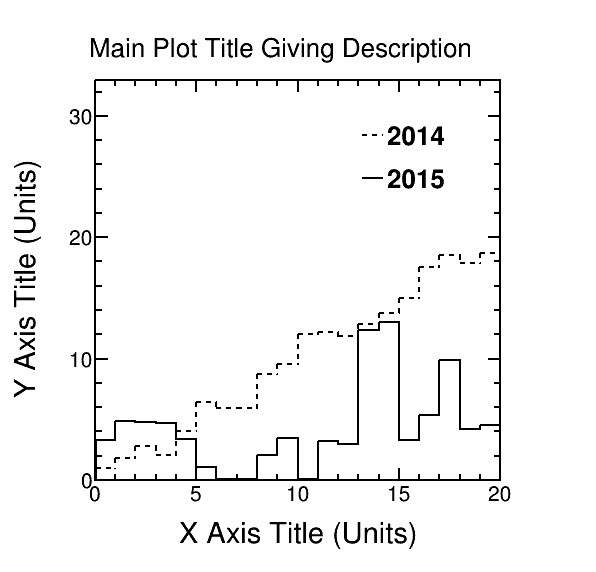
\includegraphics[scale=0.35]{pics/goodplot.png}
\end{center}
\end{frame}

\begin{frame}{Bad Plot\ldots}
\begin{center}
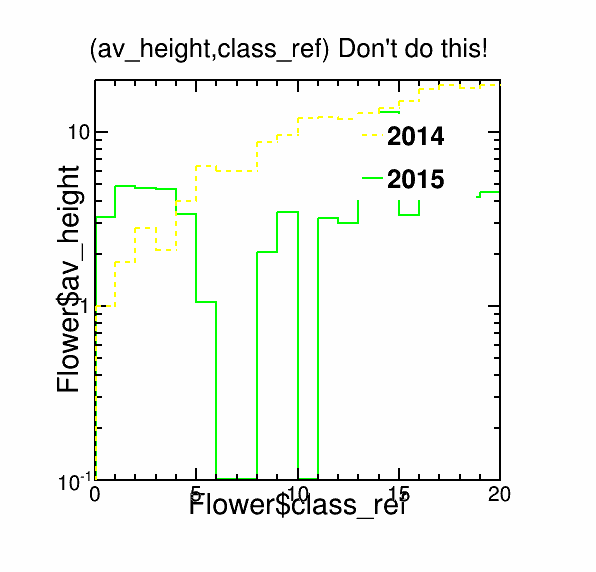
\includegraphics[scale=0.35]{pics/badplot.png}
\end{center}
\end{frame}

\begin{frame}{What does it mean to make the right plot?}

\begin{itemize}
\item Ask a good question
\item Answer the question in one plot
\end{itemize}

\end{frame}


\begin{frame}{Correlation}

Strong/Weak?

\vspace{5mm}

Direction?

\vspace{5mm}

Linear/Non-linear\ldots?

\end{frame}


\begin{frame}{How to discover correlations?}

Make some plots!!  Of course\ldots

\begin{itemize}
\item Typically make scatterplots of each pair of variables
\item Can you see a relationship?  If not then not strong.
\item Describe relationships using functions (not only linear!)
\end{itemize}

\end{frame}


\begin{frame}{Function Examples}


\begin{itemize}
\item linear, quadratic, cubic\ldots polynomial
\item exponential, logarithmic
\item Gaussian
\item etc.
\end{itemize}


\end{frame}


\begin{frame}{Why we need to be quantative\ldots}

Later on we are going to try to use some variables to predict others, this requ\
ires fitting a sensible function to the available data.

\vspace{5mm}

These problems come in two main categories:
\begin{enumerate}
\item You have a theoretical model for how the variables should be related
\item You have no theoretical model for the relationship and you have to guess somehting from the data
\item Some combination of the two due to \textit{e.~g.~}unexpected noise.
\end{enumerate}

\end{frame}




\begin{frame}{The second case: guessing functions}

Often there is not a single right answer (theme of this course\ldots)

\vspace{5mm}

Which function is good enough?
\begin{itemize}
\item Needs to describe the major features of the data
\item Should be minimal - as simple as will work
\item May well not be unique, you can try fitting different functional forms and see which one works best
\item We will start the actual fitting next week
\end{itemize}


\end{frame}


\begin{frame}{What is a feature?}


Things to look for and check match:
\begin{itemize}
\item behaviour as $x \rightarrow \pm \infty$
\item turning points (gradient = 0)
\item crossing points with the axes
\end{itemize}

\end{frame}


\begin{frame}{Types of Causation}

If A and B are correlated then there are different possibilities of causation:
\begin{itemize}
\item A causes B
\item B causes A
\item C causes A and B (lurking factor)
\item A causes C which causes B (or vice versa)
\item A causes B and B causes A (cyclic or bidirectional)
\item there is no connection between A and B only coincidence
\end{itemize}


\end{frame}





\begin{frame}{Interpolation/Prediction}

Interpolation - finding values between two known points

\vspace{5mm}

Prediction - estimating values outside the range of the data

\end{frame}



\begin{frame}{Fitting vs Interpolation}

Interpolation - when you have no or very small errors, for example in your model calculations

\vspace{5mm}

Fitting - to deal with errors in your data

\end{frame}


\begin{frame}{Regression Fitting}

We want to get a function that describes our data well, but we know there are uncertainties in the data causing some scatter in the data points

\end{frame}


\begin{frame}{Under and Over Fitting}

If you define a suitably complex function, you can get it to pass through all of your data points (like with the splines).  However, this does not mean that the features in you function really exist, rather they are probably caused by statistical noise - \textbf{over fitting}.

\vspace{5mm}

If you try to fit a straight line to a non-linear functional relationship then you will not be able to well describe the behaviour of the data - \textbf{under fitting}.

\end{frame}


\begin{frame}{Checking for under/over fitting}

\begin{enumerate}
\item Look at the data and fit and use your brain
\item Ask if the function you have used is the simplest one that could describe the data?
\item Ask if the fit describes the data well?
\item Test the fit on a subset of the data (training set)
\end{enumerate}

\end{frame}


\begin{frame}{Applying Statistics to Distributions}

\end{frame}


\begin{frame}{Experimental Design}

\end{frame}




\begin{frame}{Exam Advice}

Stay calm and think.

\vspace{5mm}

Ask yourself: does my answer make sense?


\end{frame}


\begin{frame}{Exam Advice}

Also revise statistics, writing R psuedo-code!

\end{frame}


\begin{frame}{Good Luck!}

\end{frame}



\begin{frame}{Project Presentations}

\end{frame}




%%%%%%%%%%%%% backup slides %%%%%%%%%%%%%%%%%%%%%%%%

\appendix
\newcounter{finalframe}
\setcounter{finalframe}{\value{framenumber}}

\begin{frame}{Backup Slides}
\end{frame}




\setcounter{framenumber}{\value{finalframe}}

\end{document}
